\section{Casi d'uso}

\subsection{Introduzione}
Questa sezione illustra i casi d'uso delineati a seguito dell'analisi del capitolato d'appalto, del confronto continuo con l'azienda proponente \textit{Halue S.r.l. SB} e delle attività di analisi interne condotte dal gruppo \textit{Git Happens}. \\
\\
Ciascun caso d'uso fornisce una descrizione dettagliata delle funzionalità del sistema dal punto di vista degli utenti e delle entità esterne, illustrando come la piattaforma risponde a determinate azioni o scenari operativi. \\
In conformità con quanto stabilito nel documento \textit{Norme di Progetto} (TODO: inserire sezione una volta scritta), ogni caso d'uso è identificato da un codice univoco secondo la sintassi \texttt{UC[Numero caso d'uso].[Numero sottocaso d'uso] - [Titolo]} ed è accompagnato dai diagrammi UML di riferimento e da una scheda testuale strutturata nei seguenti campi:
\begin{itemize}
    \item \textbf{Identificativo e Titolo:} codice univoco e descrizione sintetica dell'obiettivo funzionale;
    \item \textbf{Attore principale:} entità esterna che avvia e guida attivamente l'interazione con il sistema per soddisfare una propria necessità;
    \item \textbf{Descrizione:} sintesi esplicativa della funzionalità modellata;
    \item \textbf{Precondizioni:} stato in cui deve trovarsi il sistema affinché l'interazione possa avere inizio;
    \item \textbf{Postcondizioni:} stato risultante del sistema al termine della corretta esecuzione dello scenario principale;
    \item \textbf{Scenario principale:} sequenza ordinata e numerata delle azioni e risposte che conducono al raggiungimento delle postcondizioni;
    \item \textbf{Estensioni:} eventuali flussi alternativi o di gestione degli errori che deviano dallo scenario principale al verificarsi di specifiche condizioni;
    \item \textbf{User story associata:} formulazione sintetica della funzionalità dal punto di vista dell'utente, volta a chiarirne il contesto e il valore operativo.
\end{itemize}

\subsection{Attori}
Gli attori rappresentano le entità esterne (utenti umani, sistemi software o componenti temporali) che interagiscono con il sistema \textbf{Sonar}.\\
\\
Dall'analisi del dominio applicativo sono stati individuati i seguenti attori:
\begin{itemize}
    \item \textbf{Utente non autenticato:} soggetto che accede all'interfaccia web di \textbf{Sonar} senza disporre ancora di una sessione attiva, la cui interazione è limitata alla procedura di autenticazione tramite provider esterno;
    \item \textbf{Utente autenticato:} utente tecnico (sviluppatore, architetto software o \textit{Tech Lead}) che ha completato con successo l'accesso ed è associato a una specifica organizzazione (\textit{tenant}). \\
    È abilitato a registrare e gestire gli store Shopify della propria organizzazione, avviare scansioni manuali, pianificare scansioni ricorrenti, esplorare lo stato degli snapshot e navigare il grafo delle dipendenze;
    \item \textbf{Temporizzatore (Scheduler):} entità temporale di sistema che avvia automaticamente, al raggiungimento delle scadenze pianificate, i flussi di lavoro durevoli per l'esecuzione delle scansioni periodiche sugli store configurati.
\end{itemize}

\subsection{Casi d'uso}

\subsubsection{UC1 - Autenticazione}
\begin{figure}[htbp]
    \centering
    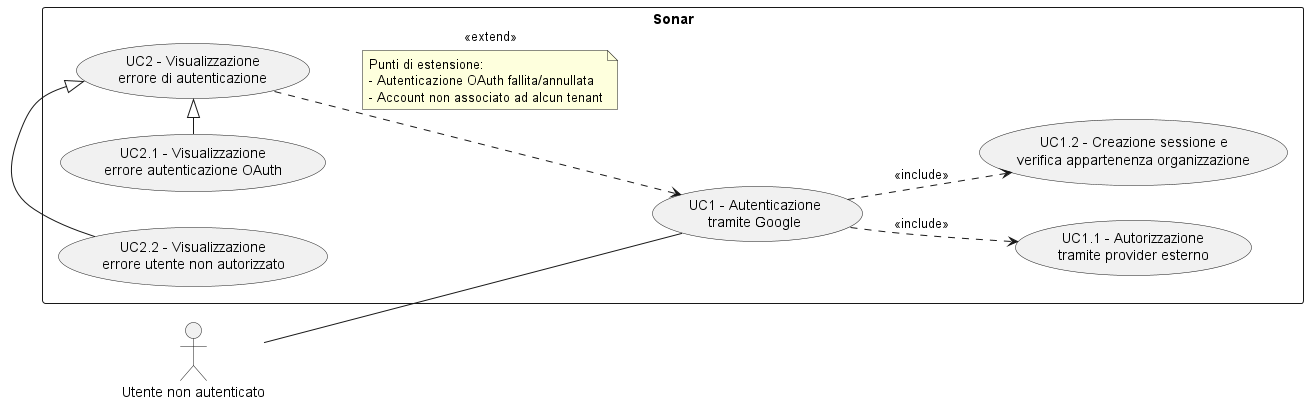
\includegraphics[width=0.9\textwidth]{assets/uc1.png}
    \caption{UC1 - Autenticazione}
    \label{fig:uc1}
\end{figure}

\begin{itemize}
    \item \textbf{Attore principale:} Utente non autenticato;
    \item \textbf{Descrizione:} L'utente effettua l'accesso alla piattaforma \textbf{Sonar} utilizzando il proprio account Google tramite il servizio di autenticazione integrato;
    \item \textbf{Precondizioni:} Il sistema è operativo e raggiungibile; l'utente non dispone di una sessione attiva;
    \item \textbf{Postcondizioni:} L'utente è autenticato, associato alla propria organizzazione (\textit{tenant}) e visualizza la dashboard degli store di competenza;
    \item \textbf{Scenario principale:}
    \begin{enumerate}
        \item L'utente accede alla schermata di login del sistema (direttamente oppure a seguito di reindirizzamento automatico da una pagina protetta);
        \item L'utente avvia la procedura selezionando l'opzione di accesso tramite Google;
        \item L'utente completa la verifica dell'identità presso il provider esterno (\textbf{include UC1.1});
        \item Il sistema istanzia la sessione di lavoro e verifica l'appartenenza dell'utente a un'organizzazione (\textbf{include UC1.2});
        \item Il sistema reindirizza l'utente alla dashboard principale mostrando esclusivamente gli store associati al suo \textit{tenant}.
    \end{enumerate}
    \item \textbf{Estensioni:}
    \begin{itemize}
        \item Autenticazione annullata dall'utente o rifiutata dal provider Google: il flusso è esteso da \textbf{UC2.1 - Visualizzazione errore autenticazione OAuth};
        \item Account Google valido ma non associato ad alcuna organizzazione censita: il flusso è esteso da \textbf{UC2.2 - Visualizzazione errore utente non autorizzato}.
    \end{itemize}
    \item \textbf{User story associata:} Come utente non autenticato voglio accedere al sistema tramite il mio account Google per consultare e gestire in sicurezza gli store della mia organizzazione.
\end{itemize}

\subsubsection{UC1.1 - Autorizzazione tramite provider esterno}
\begin{itemize}
    \item \textbf{Attore principale:} Utente non autenticato;
    \item \textbf{Descrizione:} L'utente interagisce con la schermata di consenso del provider OAuth (Google) per autorizzare l'identificazione verso \textbf{Sonar};
    \item \textbf{Precondizioni:} L'utente ha avviato \textbf{UC1} selezionando l'accesso tramite Google;
    \item \textbf{Postcondizioni:} Il provider esterno conferma l'identità dell'utente e restituisce al sistema un codice di autorizzazione valido;
    \item \textbf{Scenario principale:}
    \begin{enumerate}
        \item Il sistema reindirizza il browser dell'utente verso la pagina di autenticazione del provider Google;
        \item L'utente seleziona il proprio account Google e concede il consenso all'accesso;
        \item Il provider reindirizza l'utente all'endpoint di callback del sistema fornendo il token di autorizzazione.
    \end{enumerate}
    \item \textbf{User story associata:} Come utente non autenticato voglio autorizzare Sonar tramite il mio account Google senza dover creare nuove credenziali dedicate.
\end{itemize}

\subsubsection{UC1.2 - Creazione sessione e verifica appartenenza organizzazione}
\begin{itemize}
    \item \textbf{Attore principale:} Utente non autenticato;
    \item \textbf{Descrizione:} Il sistema valida l'identità ricevuta, avvia la sessione applicativa e associa l'utente al rispettivo \textit{tenant};
    \item \textbf{Precondizioni:} Il flusso \textbf{UC1.1} si è concluso con successo;
    \item \textbf{Postcondizioni:} La sessione dell'utente è attiva e il contesto organizzativo è stato determinato;
    \item \textbf{Scenario principale:}
    \begin{enumerate}
        \item Il sistema verifica la validità del token ricevuto tramite \textit{Supabase Auth};
        \item Il sistema interroga la base di dati per individuare l'organizzazione (\textit{tenant}) associata all'identità dell'utente;
        \item Il sistema genera i cookie/token di sessione sicuri lato client.
    \end{enumerate}
    \item \textbf{User story associata:} Come utente voglio che il sistema riconosca automaticamente la mia organizzazione al termine dell'accesso per operare nel corretto ambiente di lavoro.
\end{itemize}

\subsubsection{UC2 - Visualizzazione errore di autenticazione}
\begin{itemize}
    \item \textbf{Attore principale:} Utente non autenticato;
    \item \textbf{Descrizione:} Il sistema gestisce il mancato completamento della procedura di accesso notificando l'anomalia all'utente;
    \item \textbf{Precondizioni:} È stato avviato \textbf{UC1}, ma si è verificata un'anomalia durante l'autorizzazione o la verifica organizzativa;
    \item \textbf{Postcondizioni:} Nessuna sessione viene attivata e l'utente visualizza un messaggio diagnostico nella schermata di login;
    \item \textbf{Scenario principale:}
    \begin{enumerate}
        \item Il sistema intercetta l'interruzione o il fallimento della procedura di accesso;
        \item Il sistema impedisce l'accesso alle risorse protette e visualizza un messaggio esplicativo privo di dettagli tecnici sensibili.
    \end{enumerate}
    \item \textbf{User story associata:} Come utente non autenticato voglio essere informato in modo chiaro qualora il tentativo di accesso non vada a buon fine.
\end{itemize}

\subsubsection{UC2.1 - Visualizzazione errore autenticazione OAuth}
\begin{itemize}
    \item \textbf{Attore principale:} Utente non autenticato;
    \item \textbf{Descrizione:} Specializzazione di \textbf{UC2} relativa al rifiuto, all'annullamento o al fallimento tecnico del flusso di autenticazione presso Google;
    \item \textbf{Precondizioni:} Durante \textbf{UC1.1} l'utente ha annullato il consenso oppure il provider ha restituito un errore di autenticazione;
    \item \textbf{Postcondizioni:} L'utente viene riportato alla pagina di login con un avviso che invita a ripetere l'accesso;
    \item \textbf{Scenario principale:}
    \begin{enumerate}
        \item Il sistema rileva l'assenza di un token valido o un codice di errore nel callback OAuth;
        \item Il sistema mostra un messaggio che notifica il mancato completamento dell'autenticazione con Google.
    \end{enumerate}
    \item \textbf{User story associata:} Come utente non autenticato voglio sapere se l'accesso con Google è stato annullato o non è riuscito per poter riprovare.
\end{itemize}

\subsubsection{UC2.2 - Visualizzazione errore utente non autorizzato}
\begin{itemize}
    \item \textbf{Attore principale:} Utente non autenticato;
    \item \textbf{Descrizione:} Specializzazione di \textbf{UC2} relativa al caso in cui l'account Google sia valido, ma non risulti censito o associato ad alcuna organizzazione in \textbf{Sonar};
    \item \textbf{Precondizioni:} Il flusso \textbf{UC1.1} ha avuto esito positivo, ma durante \textbf{UC1.2} non viene trovata alcuna associazione a un \textit{tenant};
    \item \textbf{Postcondizioni:} L'eventuale sessione temporanea viene invalidata e l'utente visualizza un messaggio di accesso negato;
    \item \textbf{Scenario principale:}
    \begin{enumerate}
        \item Il sistema rileva che l'utente autenticato non appartiene ad alcun \textit{tenant} attivo;
        \item Il sistema revoca la sessione appena creata e reindirizza alla schermata di login;
        \item Il sistema visualizza un messaggio che informa l'utente che il proprio account non è abilitato ad accedere alla piattaforma.
    \end{enumerate}
    \item \textbf{User story associata:} Come utente non autorizzato voglio ricevere un avviso esplicito se il mio account Google non è associato ad alcuna organizzazione abilitata.
\end{itemize}

\subsubsection{UC3 - Disconnessione dal sistema (Logout)}

\begin{figure}[htbp]
    \centering
    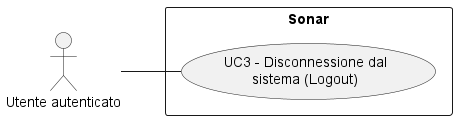
\includegraphics[width=0.9\textwidth]{assets/uc3.png}
    \caption{UC3 - Disconnessione}
    \label{fig:uc3}
\end{figure}

\begin{itemize}
    \item \textbf{Attore principale:} Utente autenticato;
    \item \textbf{Descrizione:} L'utente termina volontariamente la propria sessione di lavoro attiva all'interno della piattaforma \textbf{Sonar};
    \item \textbf{Precondizioni:} Il sistema è operativo e l'utente dispone di una sessione autenticata attiva;
    \item \textbf{Postcondizioni:} La sessione applicativa viene invalidata, i token di autenticazione lato client vengono revocati e l'utente viene reindirizzato alla schermata di login;
    \item \textbf{Scenario principale:}
    \begin{enumerate}
        \item L'utente seleziona il comando di disconnessione (\textit{logout}) dall'interfaccia web del sistema;
        \item Il sistema termina la sessione attiva tramite \textit{Supabase Auth} e rimuove i token/cookie di sessione lato client;
        \item Il sistema reindirizza l'utente alla pagina di autenticazione impedendo ulteriori accessi alle risorse protette.
    \end{enumerate}
    \item \textbf{User story associata:} Come utente autenticato voglio poter effettuare il logout per chiudere in sicurezza la mia sessione di lavoro.
\end{itemize}